\documentclass[12pt,a4paper]{article}
\usepackage[utf8]{inputenc}
%\usepackage[spanish]{babel}
\usepackage{amsmath}
\usepackage{amsfonts}
\usepackage{amssymb}
\usepackage{graphicx}
\newcommand*{\qed}{\hfill\ensuremath{\blacksquare}}
\setlength{\parindent}{0pt}
\pretolerance=2000
\tolerance=3000
\author{Santiago de Diego, Jesús Bueno, Fernando de la Cruz, Javier Ruiz}
\title{Cadenas de Markov en tiempo continuo}
\date{}
\begin{document}
\maketitle
\newtheorem{theorem}{Teorema}[section]
\newtheorem{lemma}{Lema}[section]
\newtheorem{proof}{Demostración}[section]
\newpage
\tableofcontents
\newpage
\section{Introducción}
\subsection{Cadenas de Markov}
Primero de todo, presentamos una introducción a las Cadenas de Markov de forma genérica. Como es conocido, las cadenas de Markov son procesos de corta memoria en el sentido de que solo recuerdan el último estado visitado para decidir cual sería el próximo. En procesos con larga memoria el valor que toma el proceso en cada paso depende de todo el pasado.

Formalizando el concepto, el proceso $\{\mathbb{X}_n \}_{n\in \mathbb{N}}$ con espacio de estados $E$ es una cadena de Markov si:

$$P(\mathbb{X}_{n+1}=y \, | \, \mathbb{X}_n = x_n , \ldots , \mathbb{X}_0 = x_0)=P(\mathbb{X}_{n+1}=y \, | \, {X_n=x_n})$$

Este tipo de procesos estocásticos tienen mucho interés a la hora de modelar determinados fenómenos, como por ejemplo el tiempo de espera a un servidor en función de la tasa de llegada de los clientes.

\subsection{Diferencia entre tiempo discreto y tiempo continuo}
La principal diferencia entre cadenas de Markov en tiempo discreto y tiempo continuo es, como dice el propio nombre, el tiempo. En las cadenas de Markov en tiempo continuo, consideramos un $t\in T \subset \mathbb{R}$ mientras que en las cadenas de Markov en tiempo discreto, trabajamos con instantes de tiempo de la forma $t\in \mathbb{N}$.
\section{Definición y propiedades}



\subsection{Relación con la teoría de autómatas}
En concreto, podemos asociar a una cadena de Markov un grafo, como veremos más abajo. De esta forma, el grafo resultante se comporta de igual manera que un \textbf{autómata finito}, relacionándose de esta forma las cadenas de Markov con la teoría de autómatas.
\\\\
Presentamos primero un concepto preeliminar que resulta imprescindible para comprender lo siguiente:
\\\\
\textbf{Definición: cadena de Markov homogénea en tiempo continuo}
\\
Una CMTC se dice homogénea si la probabilidad de ir del estado $i$ al estado $j$ no depende del instante de tiempo en el que se encuentra la cadena, formalmente esto es:
$$P(\mathbb{X}_n=j \, | \, \mathbb{X}_{n-1}=i)=P(\mathbb{X}_1=j \, | \, \mathbb{X}_0=i)$$
Una vez entendido este concepto introducimos por tanto la siguiente definición:
\\\\
\textbf{Definición: Grafo asociado a una CMTC-h}
\\
$G=(E,U,W)$ es el grafo asociado a una CMTC homogénea sii:
\begin{itemize}
\item $E$ es el conjunto de estados de la cadena
\item $U$ es el conjunto de aristas, que en este caso sería el conjunto de transiciones posibles
\item $W$ es el conjunto de ponderaciones. Podemos verlo como el conjunto de valores de cada arista
\end{itemize}
Además $G$ es un grafo orientado, es decir, que tenemos en cuenta cual es el nodo origen y cual es el nodo destino.
\\\\
Una vez presentada la definición de grafo asociado a una CMTC-h, podemos establecer una biyección entre el conjunto de grafos orientados asociados a una CMTC-h y el conjunto de los autómatas finitos deterministas, aunque estos resultados se escapan del alcance del trabajo en cuestión. Simplemente mostraremos un ejemplo de uno de estos grafos:
\\
\begin{figure}[h]
  \centering
    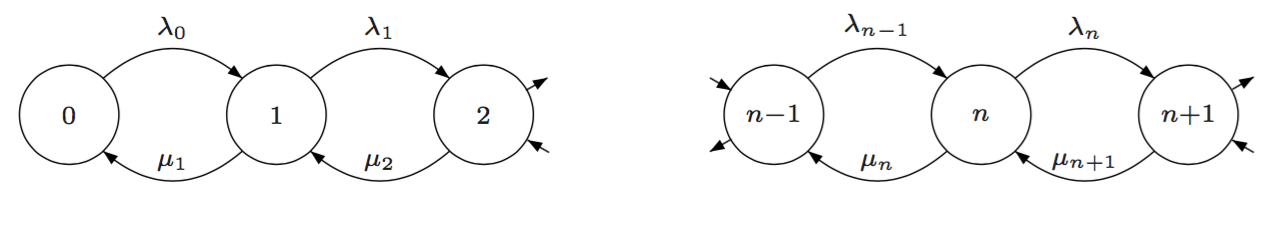
\includegraphics[width=0.7\textwidth]{img/grafo.png}
  \caption{Ejemplo de grafo de una CMTC-h}
  \label{fig:ejemplo}
\end{figure}

\section{Probabilidades de transición}
\section{Ecuación de Kolmogorov}
\section{Clasificación de los estados}
\section{Teoremas límite}
\section{Ejemplos}
\subsection{Ejemplo 1}
\subsection{Ejemplo 2}
\end{document}}